
%%This is a very basic article template.

%%There is just one section and two subsections.

\documentclass[12pt]{article}

\usepackage[slovak]{babel}
\usepackage[utf8]{inputenc}
\usepackage{amsmath}
%%\usepackage[dvipdfm]{graphicx}
\usepackage{graphicx}
\usepackage{bmpsize}
\usepackage{pdfpages}
\usepackage{wrapfig}
\usepackage{setspace}
\usepackage[top=2.54cm, bottom=2.54cm, left=3.5cm, right=2.0cm]{geometry}

\setstretch{1.5}

\begin{document}

\title{Rozpoznávanie dopravných značiek}

\author{Mário Kapusta}
%% titulka s informaciami
\maketitle
\thispagestyle{empty}
\clearpage
%% obsah
\tableofcontents
\addtocontents{toc}{\protect\thispagestyle{empty}}
\thispagestyle{empty}
\clearpage
%%zoznam tauliek
\listoftables
\thispagestyle{empty}
\clearpage
%%zoznam orazkov
\listoffigures
\thispagestyle{empty}
\clearpage
%% astrakt
\begin{abstract}
V praci sme sa zaoberali
\end{abstract}
\clearpage

%% zaciatok prace
\section{Počítačové videnie}
Nejaký obkec o počítačovom videní
\subsection{História počítačového videnia}
Niečo krátke o histórii počítačového videnia
\subsection{Hlavné témy počítačového videnia}
Obkec o rozdelení počítačového videnia a rôznych odvetviach venovania
\subsubsection{Transformácia}
Niečo o trnaformácii.
\subsubsection{Filtrovanie a kompresia}
Niečo o kompresii.
\subsubsection{Vylepšovanie obrazu}
Niečo o vylepšovaní obrazu.
\subsubsection{Rozpoznávanie objektov}
Niečo o rozpoznávaní objektov
\subsubsection{Pozíciovanie}
Niečo o rozpoznávaní poziciovani
\subsection{Technológie}
Niečo o o technológiách rozpoznávania vo všeobecnosti
\subsubsection{OpenCV}
Niečo o opencv - textik k tomu:
http://simplecv.tumblr.com/post/19307835766/opencv-vs-matlab-vs-simplecv
\subsubsection{Matlab}
Niečo o matlabe
\subsubsection{SimpleCV}
Niečo o simplecv

\section{Rozpoznávanie ojektov}
\section{OpenCV, Android a Java - inak to nazvat}
\paragraph{}
Cieľom práce je vypracovať komplexný návrh riešenia pre vyhľadávanie a rozpoznávanie dopravného značenia a taktiež vytvoriť funkčnú aplikáciu, ktorá
bude schopná rozpoznať zvislé dopravné značenia. Táto aplikácia bude naprogramovaná v jazyku Java a bude spustiteľná na
 operačnom systéme Android 2.3, ktorý je určený pre mobilné zariadenia. Computer vision (počítačové videnie), nám zaručí open-source knižnica OpenCV.
\subsection{Matematická terminológia}
\paragraph{}
Mnoho matematických metód sa bude priamo vysvetlovať pri predstavovaní danej OpenCV funkcionality.
V tejto sekcii si predstavíme také matematické metódy ktoré nám pomůžu lepšie sa orientovať pri opise konkrétnych funkcionalít OpenCV.
\subsubsection{Konvolúcia}
\paragraph{}
Konvolúcia je matematická metóda, ktorá systematicky prechádza celý obraz a na výpočet novej hodnoty bodu využíva malé okolie O reprezentatívneho bodu. 
Táto hodnota je zapísaná do nového obrazu. Diskrétna konvolúcia má tvar:
\begin{align*}
g(x,y) = \sum_{(m,n)} \sum_{(e^0)} h(x - m,y - n)f(m,n)
\end{align*}
kde f predstavuje obrazovú funkciu pôvodného obrazu, g predstavuje obrazovú funkciu nového obrazu, h predstavuje konvolučnú masku alebo konvolučné jadro, h nám udáva koeficienty jednotlivých bodov v okolí O.
Najčastejšie sa používajú  obdĺžníkové masky s nepárnym počtom riadkov a stĺpcov, pretože v tom prípade môže reprezentatívny bod ležať v strede masky.
\paragraph{}
Transformácie v lokálnom okolí bodu sa delia na dve skupiny: \\
\textbf{Vyhladzovanie} – tieto metódy sa snažia potlačiť šum v obraze, ale rozostrujú hrany. \\
\textbf{Ostrenie} – detekcia hrán a čiar, ale zosilňuje šum. \\
\paragraph{}
Podľa matematických vlastností môžeme metódy predspracovania rozdeliť na \\
\textbf{Lineárne metódy} – novú jasovú hodnotu bodu počítajú ako lineárnu kombináciu vstupných bodov. Napr.: priemerovací filter \\
\textbf{Nelineárne metódy} – berú do úvahy len body s určitými vlastnosťami. Napr.: mediánový filter.
\cite{DIP}
\subsection{Funkcionalita OpenCV}
\paragraph{}
OpenCV je open source knižnica počítačového videnia. Knižnica je napísaná v programovacích jazykoch C a C++. Aktívne sa pracuje na
rozhraniach pre Python, Ruby, Matlab, Javu a iných programovacích jazykoch. V našej práci sme sa sústredili na verziu pre programovací jazyk Java,
ktorý sa používa pri tvore aplikácii pre Android OS.
\cite{learning_opencv}
\paragraph{}
OpenCV knižnica bola navrhnutá tak, aby funkcie použité v tejto knižnici, boli čo najefektívnejšie a čo najviac zamerané na real-time aplikácie.
Knižnica je napísaná v optimalizovanom jazyku C a tak môže jednoducho využiť aj silu viacjadrových procesorov.
Taktiež existujú knižnice, špeciálne určené pre procesory s architektúrou Intel. IPP (Integrated Performance Primitives) knižnice  sa skladajú z nízko levelových 
optimalizovaných postupov a rôznych algoritmických olastí, ktoré pracujú na procesoroch s architektúrou Intel oveľa efektívnejšie.
\cite{learning_opencv}
\paragraph{}
Jeden z hlavných cieľov OpenCV je sprístupniť jednoducho použiteľné prostredie ktoré pomôže developerom ľahko a rýchlo budovať aplikácie s použitím počítačového videnia
pre rôzne použitia v oblasti, medicíny, bezpečnosti, robotiky, dopravy, priemyselnej výroby a iných, pre ktoré ma OpenCV dokonca aj špecifické funkcionality.
\cite{learning_opencv}
\paragraph{}
Pre olasť rozpoznávania ojektov sú taktiež mnohé špecifické funkcionality.
Pri problematike rozpoznávania zvislích dopravných značení sme niektoré z nich použili a preto je potrebné si pre lepšie pochopenie problematiky tieto funkcie vysveliť podrobnejšie.
\subsubsection{cvtColor}
\paragraph{}
Funkcia \emph{cvtColor} prevedie obraz z jedného farebného spektra do iného. Je to jedna z najpoužívanejších funkcií, keďže na rozpoznávanie objektov je potrené si obraz pripraviť
cez mnohé farebné filtre. Vstupné parametre je možné pozorovať pri tabuľke \ref{cvtColorPar}.
\cite{cvtColor}
\cite{OpenCVDoc}
\begin{table}
	\centering
    \begin{tabular}{ | l | l | p{5cm} |}
    \hline
    Premenná & Dátový typ & Popis \\ \hline
    src & Mat & Vstup je 8-bitový, 16-bitový obraz alebo formát čísla s plávajúcou desatinou čiarkou. \\ \hline
    dst & Mat & Výstupný obraz s rovnakými parametrami ako na vstupe. \\ \hline
    code & int & Farebné spektrum ktoré do ktorého požadujeme obraz previesť. \\
    \hline
    \end{tabular}
  	\caption{Tabulka znázorňuje vstupy funkcie cvtColor}
  	\label{cvtColorPar}
\end{table}
\paragraph{}
Pri používaní funkcie \emph{cvtColor}, je potrebné si určiť o akú konverziu ide. OpenCV, už má k dispozícii predpripravené konštanty, ktoré konverziu lepšie vyjadrujú.
Matematický prepočet si OpenCV už spraví v jadre. Konverzií je v OpenCV naprogramovaných už mnoho, my si predstavíme matematický model konverzie,
ktorú v našom prípade rálne využijeme. Jedná sa o konverziu z BGR(pri OpenCV je poradie kanálov pre model RGB zoradený opačne) do farebného modelu HSV a späť.
\cite{cvtColor}
\cite{OpenCVDoc}
\paragraph{} 
V prípade 8 a 16 bitového obrazu je potrené jednotlivé kanály R,G a B previesť do formátu s plávajúcou desatinou čiarkou a zmenšiť rozsah od 0 do 1.
\begin{table}
\begin{align*}
BGR \leftrightarrow HSV
\end{align*}
\begin{align*}
V \leftarrow max(R,G,B)
\end{align*}
\begin{align*}
S \leftarrow \begin{cases} \frac{V - min(R,G,B)}{V}, & \text{ pokiaľ } V \neq 0 \\ 0, & \text{ pokiaľ } V = 0 \end{cases} \\
\end{align*}
\begin{align*}
H \leftarrow \begin{cases} \frac{60(G - B)}{V - min(R,G,B)}, & \text{ pokiaľ } V = R \\ \frac{120 + 60(B - R)}{V - min(R,G,B)}, & \text{ pokiaľ } V = G \\ \frac{240 + 60(R - G)}{V - min(R,G,B)}, & \text{ pokiaľ } V = B \end{cases} 
\end{align*}
\begin{align*}
\text{ Pokiaľ } H < 0, & \text{ tak } H = H + 360
\end{align*}
\begin{align*}
\text{ Na výstup pôjde } 0 \le V \le 1, 0 \le S \le 1, 0 \le H \le 1
\end{align*}
\caption{Konverzia RGB modelu na HSV\cite{hsv_wiki_cz}\cite{cvtColor}\cite{OpenCVDoc}}
\label{cvtColorEquals}
\end{table}
\subsubsection{Canny}
\paragraph{}
Hlavná úloha funkcie \emph{Canny} je vyhľadávať okraje, kontúry a hrany všetkých objektov. Pri kombinácii s rôznymi filtrami, môžeme docieliť, vyhľadanie hrán úmyselného objektu.
Na rozoznávanie sa využíva algoritmus \emph{Canny86}.
\cite{canny}
\cite{OpenCVDoc}
\paragraph{}
Kontúrový alebo hranový detektor by mal spĺňať tri kritéria, ktoré určil John Canny.
\begin{enumerate}
  \item Detekčné kritérium, detektor nesmie zabudnúť na významnú hranu a na jednu hranu môže byť maximálne jedna odozva.
  \item Lokalizačné kritérium, rozdiel medzi skutočnou a nájdenou hranou má byť minimálny.
  \item Kritérium jednej odozvy.
\end{enumerate}
Cannyho detektor využíva konvolúciu s dvojrozmerným Gaussianom a deriváciu v smere gradientu.
Poskytuje informácie o smere a veľkosti hrany. Nech G je dvojrozmerný Gaussian. Nech Gn je prvá derivácia G v smere gradientu
\begin{align*}
G_n = \frac{\delta G}{\delta n} = n\bigtriangledown G
\end{align*}
kde n je smer gradientu, ktorý dostaneme nasledovne
\begin{align*}
n = \frac{\bigtriangledown(G * f)}{|\bigtriangledown(G * f)|}
\end{align*}
Hranu dostaneme v bode, kde funkcia \begin{math}\ G_n *f  \end{math} dosiahne lokálne maximum, a druhá derivácia sa rovná nule.
\begin{align*}
\frac{\delta^2}{\delta n^2} G * f = 0
\end{align*}
Pre silu hrany platí:
\begin{align*}
|G_n * f| = |\bigtriangledown (G * f)|
\end{align*}
Kritérium jednej odozvy sa dosahuje následne prahovaním. 
\cite{DIP}
\cite{JCanny}
\cite{canny_wiki_en}
\paragraph{}
Vstupné parametre je možné pozorovať pri tabuľke \ref{cannyPar}.
Najmenšia hodnota medzi \emph{threshold1} a \emph{threshold2} je použitá na prepájanie kontúr. Tá najväčšia hodnota je použitá ako začínajúci segment najsilnejších kontúr.
Pri správnom nastavení, sa dá dosiahnuť pomerne kvalitné odstránenie nepotrených kontúr.
\cite{canny}
\cite{OpenCVDoc}
\begin{table}
	\centering
    \begin{tabular}{ | l | l | p{5cm} |}
    \hline
    Premenná & Dátový typ & Popis \\ \hline
    image & Mat & Vstup je 8-bitový obraz s jedným farebným kanálom. \\ \hline
    edges & Mat & Výstup je mapa všetkých nájdených kontúr. \\ \hline
    threshold1 & double & Prvá prahová hodnota (threshold). \\ \hline
    threshold2 & double & Druhá prahová hodnota (threshold). \\
    \hline
    \end{tabular}
  	\caption{Tabulka znázorňuje vstupy funkcie canny}
  	\label{cannyPar}
\end{table}
%%\subsubsection{HoughLinesP}
%%nebolo v praci pouzite
\subsubsection{GaussianBlur}
\paragraph{}
Vyhladzuje obraz pomocou \emph{GaussianBlur} filtra.
\cite{gaussianblur_doc}
\cite{OpenCVDoc}
\emph{GaussianBlur} filter funguje na princípe \emph{N x N} konvolúcie pri ktorej sa každý pixel prehodnotí na základe \emph{Gaussian} funkcie.
Táto funkcia tak prevedie rozostrenie pre každý pixel obrazu.
\cite{gaussianblur}
\begin{align*}
H(x,y) = \frac{1}{2\pi\sigma^2}e^{\frac{(x^2)+(y^2)}{2\sigma^2}}
\end{align*}
\paragraph{}
Princíp konvolúcie 2D obrazu je postavený na tom, že sa systematicky snažíme spracovávať okolie pixelu a dostať výslednú hodnotu z okolia reprezentatívneho bodu.
Konvolúcia sa často používa pri spracovávaní obrazu, ako je vyhladzovanie obrazu, ostrenie, detekcia hrán a obrázkov.
\cite{convolution}
\cite{DIP}
\paragraph{}
Vstupné parametre pre \emph{GaussianBlur} je možné pozorovať pri tabuľke \ref{gaussianblurPar}. 
Pri premennej \emph{ksize} si môžeme napríklad nastaviť veľkosť matice, ktorá sa bude pri konvolúcii používať.
Veľkosť matice pri konvolúcii ovplivní rozostrenie. Čím väčšiu maticu používame, tím väčšie rozostrenie dostaneme.
\cite{gaussianblur_doc}
\cite{OpenCVDoc}
\begin{table}
	\centering
    \begin{tabular}{ | l | l | p{5cm} |}
    \hline
    Premenná & Dátový typ & Popis \\ \hline
    src & Mat & Vstup je obraz s ľubovolným počtom farebných kanálov. \\ \hline
    dst & Mat & Výstup s rovnakými parametrami ako bol vstup. \\ \hline
    ksize & Size & Veľkosť Gaussian jadra. Matica konvolúcie. \\ \hline
    sigmaX & double & Smerodajná odchýlka Gaussian jadra v smere X. \\ \hline
    sigmaY & double & Smerodajná odchýlka Gaussian jadra v smere Y. \\
    \hline
    \end{tabular}
  	\caption{Tabulka znázorňuje vstupy funkcie GaussianBlur}
  	\label{gaussianblurPar}
\end{table}
\subsubsection{inRange}
\subsubsection{threshold}
\subsubsection{bitmapToMat}
\subsubsection{findContours}
\subsubsection{boundingRect}
\subsubsection{drawContours}
\subsubsection{contourArea}
\subsubsection{fitEllipse}

\section{Návrh riešenia}
\paragraph{}
Po dôkladnom naštudovaní literatúry a potrebných algoritmov je našim cieľom vyhotoviť riešenie, ktoré by dokázalo detekovať zvislé dopravné značenia.
Návrh bude pozostávať z návrhu algoritmov, návrhu objektov a návrhu užívateľského prostredia.
\subsection{Návrh algoritmov}
\paragraph{}
Ako metódu rozpoznávania som si zvolil detekciu dopravného značenia podľa tvaru a farby. 
Algoritmy ktoré som navrhol, sú postavené na princípe rozpoznania farebného rozhrania hľadaného objektu a následné detekovanie potrebného tvaru.
Pri opise som sa zameral na detekciu značiek, ktoré sú na cestách najviac početné.
Na cestách prevládajú dopravné značenia, ktoré sú červenej a modrej farby. Z tvarov prevládajú kruhy a trojuholníky.
Samotné rozpoznanie bolo uskutočnené pomocou neurónových sietí. Táto metóda je najlepšia na počítačové učenie objektov.
Na rozdiel od detekcie dopravného značenia, pre riešenie neurónových sietí použijeme už existujúcu knižnicu.
\subsubsection{Návrh algoritmu pre detekciu farby}
%%TODO Spravenie vyvojoveho/stavoveho diagramu
\paragraph{}
Ako prvý algoritmus som si vybral detekciu červenej farby. Pre detekciu farieb sa v literatúre odporúča najprv previesť vstup na farebný model HSV. 
Vstup prichádza vo farebnom formáte RGB. Farebný model HSV je jeden z dvoch najpoužívanejších valcovo súradnicových reprezentácii bodov pre RGB model.
\cite{hsl_hsv_wiki_en}
\paragraph{}
Na začiatok by sa mal vstup(bitmapa) konvertovať na binárnu maticu.
\paragraph{}
Najväčšia výhoda dopravného značenia je, že je silne kontrastné od ostatného prostredia.
Túto vlastnosť môžeme perfektne využiť v náš prospech a pomocou pomocou rozmazania obrazu, môžeme dosieliť to,
že sa zbavíme slabších kontú hneď na začiatku. V OpenCV je pre rozmazávanie obrazu na výber viacero metód,
no my použijeme matódu \emph{GaussianBlur}, ktorá už názvom prezrádza použitie známeho filtra \emph{Gaussian blur}
\paragraph{}
Keďže sa snažíme dostať náš vstupný obraz do formátu HSV, o ktorú sa stará funkcionalita \emph{cvtColor} 
potrebujeme mu nastaviť vstup tak, aby obraz vedel bez problémov spracovať. 
Keďže na väčšine mobilných zariadení prichádza do zariadenia obraz vo formáte RGBA, ďalší krok bude nepríklad konvertovanie formátu RGBA na formát RGB.
\paragraph{}
Ďalej bude nasledovať samotná konverzia obrazu do HSV pomocou už spomínanej metódy \emph{cvtColor}.
\paragraph{}
Ďalší krok bude spracovať každý kanál farebného modelu HSV samostatne. Ako prvý spracujeme \emph{Hue} kanál, ktorý sa stará o farebný odtien každého pixelu.
\emph{Hue} Farba sa v tomto kanáli určuje podľa stupňov. 
Primárne sa začína na stupni 0$^\circ$, čo predstavuje zelenú farbu, postupne prechádza do modrej,
ktorá sa nachádza na 120$^\circ$ stupňoch z kade prechádza cez červenú na 240$^\circ$ a keďže je to model kruhový, vracia sa do zelenej na 360$^\circ$.
Pomocou funkcie \emph{inRange} by nemal byť problém určiť rozhranie stupňov, ktoré sme schopný akceptovať ako hľadanú farbu pre hľadané naše dopravné značenia.
Ďalší kanál je \emph{Saturation}, ktorý predstavuje sýtosť farby. Táto sýtosť sa vyjadruje v percentách, kde 0\% predstavuje šedú a 100\% je plne sýta farba.\cite{hsv_wiki_cz} 
V našom prípade je postacuje metóda \emph{threshold}. Posledný kanál \emph{Value} vyjadruje hodnotu jasu.
Keďže v praxi znamená znižovanie jasu pridávanie čiernej do základnej farby,
pre hľadanie červenej farby na dopravnom značení nie je potrebné s týmto kanálom pracovať, lebo červená farba použitá na dopravných značeniach je pomerne svetlá.
Pri hľadaní modrej je túto farbu potrebné trochu stmaviť a tak použijeme opäť funkciu \emph{threshold}.
\paragraph{}
Na koniec potrebujeme dostať len kontúry hľadanej farby. 
Najpr si budeme musieť spojiť jednotlivé kanály späť do jednej binárnej matice použitím metódy \emph{Canny}. 
Po tomto kroku by nám mali ostať len čierny obraz a biele škvrny predstavujúce červenú farbu v požadovanom rozsahu.
Z týchto bielych objektov, budeme potrebovať len okraje a tak použijeme metódu \emph{findContours}, ktorá sa postará o to, že dostaneme pole kontúr z celého obrazu.
S týmito kontúrami potom ďalej pracujeme a rozoznávame z nich hľadané útvary.
\subsubsection{Návrh algoritmu pre detekciu kruhov}
\paragraph{}
Pri detekcii dopravného značenia v tvare kruhu, je dôležité počítať s tým, že nehľadáme úplný kruh. Kruhové dopravné značenia sú vyrábané ako dokonalý kruh,
no pri ich rozpoznávaní si je potrené uvedomiť, že na objekt sa pozeráme z rôznych uhlov. Táto skutočnosť nám prináša do prolematiky dôležitý fakt,
že v skutočnosti to nie sú kruhy čo hľadáme, ale sú to elipsy. Celý algoritmus je možné vidieť na orázku č. \ref{hladanie_kruhov}

%% otekanie textu
%%\begin{wrapfigure}{r}{0.55\textwidth}
%%	\begin{center}
%%		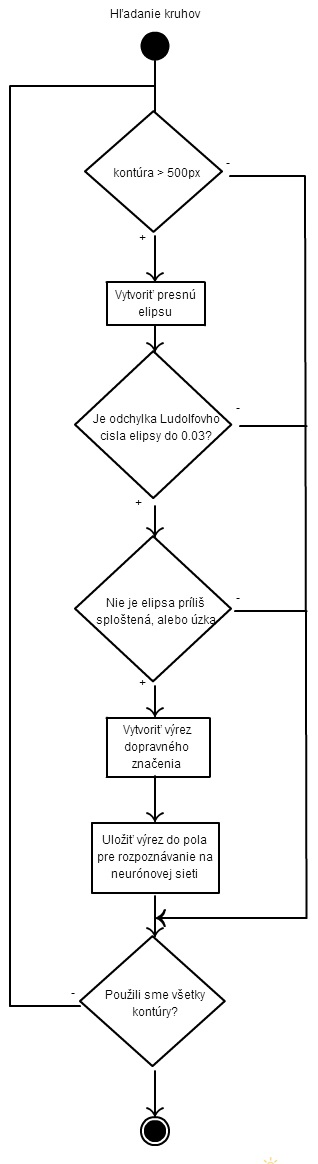
\includegraphics[width=0.4\textwidth,natwidth=318,natheight=1164]{hladanie_kruhov.jpg}
%%	\end{center}
%%	\vspace{-20pt}
%%  	\caption{Algoritmus vyhľadávania kruhov}
%%  	\vspace{-10pt}
%%  	\label{hladanie_kruhov}
%%\end{wrapfigure}
\begin{figure}[p]
\centering
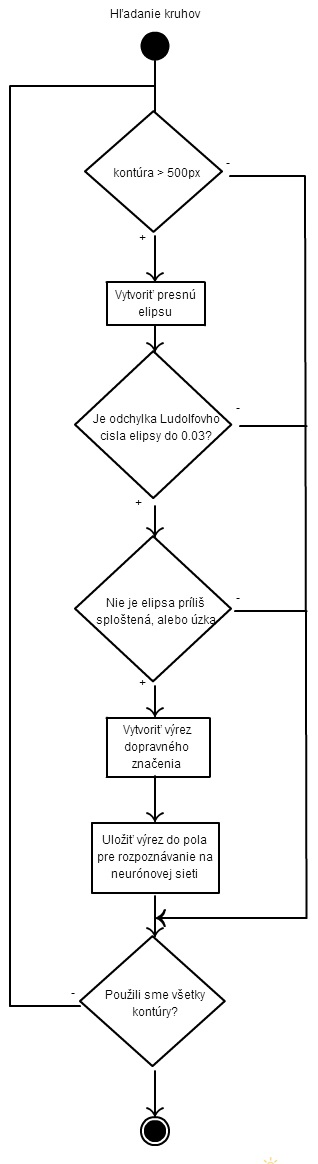
\includegraphics[width=0.38\textwidth,natwidth=318,natheight=1164]{hladanie_kruhov.jpg}
\vspace{-20pt}
\caption{Algoritmus vyhľadávania kruhov}
\vspace{-10pt}
\label{hladanie_kruhov}
\end{figure}

\paragraph{}
Keďže v predchádzajúcej kapitole sme si navrhli riešenie, ktoré nám vracia len kontúry hľadanej farby, môžeme pokračovať od tohto bodu.
Ako prvé si spravíme cyklus, ktorým budeme prechádzať všetky naše vyhľadané kontúry farieb. Aby sme eliminovali počet prebytočných kontúr, 
je potrené spracovávať čo najrelevantnejšie výsledky. Tento úkon vykoná metóda \emph{contourArea}, vďaka ktorej budeme posielať na ďalšie spracovanie len kontúry väčšie ako 500 pixelov.
\paragraph{}
Vzhľadom na to, že výsledky, ktoré dostávame ešte nemôžeme nazvať elipsami, musíme si naše kontúry na elipsy upraviť.
Tento úkon vykonáva metóda \emph{fitEllipse}, ktorá upraví kostrbaté kontúry, ktoré sa aspoň trochu podobajú elipse, na matematicky presnú elipsu.
\linebreak
\linebreak
\paragraph{}
Keď už máme detekované elipsy, nastáva posledný krok, a tým krokom je, určiť si toleranciu elipsy dopravného značenia, ktorú vyhľadávam.
Táto tolerancia, je vlastne tolerancia nepresnosti, pri výpočte Ludolfovho čísla. 
Ďalším krokom je tak výpočet už spomínaného ludolfovho čísla a následné overenie jeho nepresnosti. 
Pokiaľ je výsledná hodnota vyhovujúca, nájdený objekt vyrežeme, a zasielame na rozpoznanie neurónovej sieti, ktorá zistí o akú značku sa presne jedná.
\paragraph{}
Výpočet Ludolfovho čísla:
\begin{align*}
          \pi = \frac{o}{d} \\
\end{align*}
Úprava výpočtu Ludolfovho čísla pre elipsu:
\begin{align*}
          p = \frac{o}{d} = \frac{o}{(\frac{1}{2} y) * ( \frac{1}{2} x)} \\
\end{align*}
Získanie tolerancie:
\begin{align*}
          \pi - p < 0.03 \\
\end{align*}
%%vzorec
%%citacie z knih matematiky
\paragraph{}
Pre určovanie tolerancie elipsy, je možné použiť ešte jednu metódu, a tou je overovanie podľa osí. 
Pokiaľ je x-ová os dvoj-násobne väčšia ako y-ová, ide už o elipsu, ktorú by sme ďalej len ťažko identifikovali. 
Takýto nežiaduci stav môže nastať, pokiaľ sa na značku pozeráme na dopravné značenie z príliž veľkého uhlu.
\paragraph{}
Dva nežiaduce stavy tvaru dopravného značenia:
\begin{align*}
		  \text{ 1.) }
          \frac{\frac{1}{2} x}{\frac{1}{2} y} > 2  \\
          \text{ 2.) }
          \frac{\frac{1}{2} y}{\frac{1}{2} x} > 2  \\
\end{align*}
\subsubsection{Návrh algoritmu pre detekciu trojuholnikov}
\subsubsection{Návrh algoritmu pre detekciu štvorcov}
\subsection{Návrh objektov - UML}
\subsection{Návrh užívteľského prostredia}

\section{Implementácia}
\subsection{Inštalácia Opencv pre Android}
\subsection{Android aplikácia a GUI}
\subsection{Objekty}
\subsubsection{Trieda 1}
\subsubsection{Trieda 2}
\subsubsection{Trieda 3}

\section{Výsledky aplikácie}
\subsection{Detekcia kruhových značiek}
\subsubsection{Značky modrej farby}
\subsubsection{Značky červenej farby}

\section{Záver}

\bibliography{bach}
\bibliographystyle{plain}

\end{document}
